

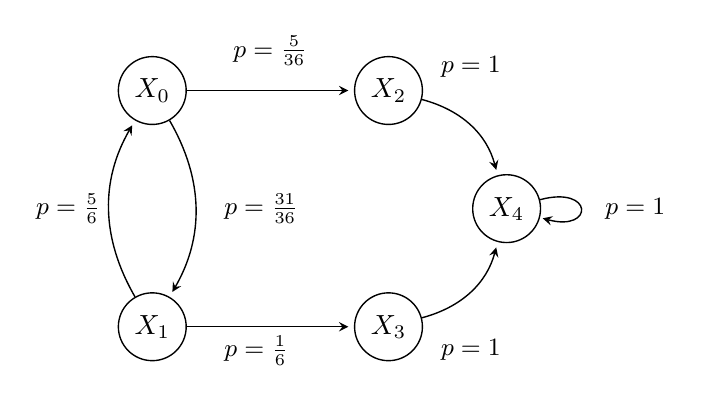
\begin{tikzpicture}[->, >= stealth, shorten >=2pt, line width=0.5pt, node distance=2cm]
  \node[circle, draw] (A) at (0, 3) {$X_0$};
  \node[circle, draw] (B) at (0, 0) {$X_1$};
  \node[circle, draw] (C) at (3, 3) {$X_2$};
  
  \node[circle, draw] (D) at (3, 0) {$X_3$};
  \node[circle, draw] (E) at (4.5, 1.5) {$X_4$};
  
  
  \begin{small}
    \path (A) edge [bend left]  node [left][right=0.25cm] {$p = \frac{31}{36}$} (B);
     \path (B) edge [bend left] node [left] {$p = \frac{5}{6}$} (A);
      \path (A) edge  node [left][above=0.2cm] {$p = \frac{5}{36}$} (C);
       \path (B) edge  node [left][below=0.3cm][right=-0.7cm] {$p = \frac{1}{6}$} (D);
        \path (C) edge [bend left] node [left][above=0.5cm] {$p = 1$} (E);
         \path (D) edge [bend right] node [left][below=0.5cm] {$p = 1$} (E);
         \path (E) edge [loop right] node [left] [right=0.2cm]{$p = 1$} (E);
   % \path (A) edge [bend left] node [below = 0.4cm] {$p = \frac{31}{36}\times\frac{5}{6}\times\frac{5}{36}$} (B);
    %\path (A) edge [bend right] node [below = 0.2cm] {$p = \frac{31}{36}\times\frac{5}{36}\times\frac{31}{36}$} (C);
    
    
  \end{small}
\end{tikzpicture}
